\documentclass[a4paper, 12pt]{report}

\usepackage{charter}
\usepackage{makeidx}
\usepackage{fancyhdr}
\usepackage{hyperref}
\usepackage[utf8]{inputenc}
\usepackage{graphicx}
\usepackage[left=2cm, right=2cm]{geometry}
\usepackage{latexsym}
\usepackage{amsmath, amsthm, amssymb}
\usepackage{rotating}


\begin{titlepage}
\title{Documento di Analisi}
\author{Release 0.8}
\date{\today \\Firenze \\\begin{figure}[h] \centering

\includegraphics[width=0.2\textwidth]{../../images/logokiwi.png} \end{figure} }
\end{titlepage}

\pagestyle{fancy}

\begin{document}

\maketitle

\section*{Approvazione, redazione, lista distribuzione}
\begin{table}[h!]
  \begin{center}
    \begin{tabular}{| l | l | p{60mm} |}
    \hline
    \textbf{approvato da} & \textbf{il giorno} & \textbf{firma} \\
	\hline    
	Marco Tinacci & \today &  \\
    \hline
    \end{tabular}
  \end{center}
\end{table}

\begin{table}[h!]
  \begin{center}
    \begin{tabular}{| l | l | p{60mm} |}
    \hline
    \textbf{redatto da} & \textbf{il giorno} & \textbf{firma} \\
    \hline
    Francesco Calabri & \today &  \\
    \hline
	Manuele Paulantonio & \today &  \\
    \hline    
	Massimo Nocentini & \today &  \\
    \hline
    \end{tabular}
  \end{center}
\end{table}

\begin{table}[h!]
  \begin{center}
    \begin{tabular}{| l | l | p{60mm} |}
    \hline
    \textbf{distribuito a} & \textbf{il giorno} & \textbf{firma} \\
	\hline    
	Daniele Poggi & \today &  \\
    \hline
	Niccol\'o Rogai & \today &  \\
    \hline
	Marco Tinacci & \today &  \\
    \hline
    \end{tabular}
  \end{center}
\end{table}

\tableofcontents

\newpage

\section*{Introduzione}
Descrizione dell'acronimo: \textbf{cdns} sta per ''\textbf{c}ome
\textbf{d}escritto \textbf{n}ella \textbf{s}pecifica''.

\part{Requisiti del prodotto}

\documentclass[a4paper, 12pt]{report}

\usepackage{charter}
\usepackage{makeidx}
\usepackage{fancyhdr}
\usepackage{hyperref}
\usepackage[utf8]{inputenc}
\usepackage{graphicx}
\usepackage[left=2cm, right=2cm]{geometry}
\usepackage{latexsym}
\usepackage{amsmath, amsthm, amssymb}
\usepackage{rotating}


\begin{titlepage}
\title{Requisiti del Prodotto}
\author{Release 0.4}
\date{\today \\Firenze \\\begin{figure}[h] \centering

\includegraphics[width=0.2\textwidth]{../images/logokiwi.png} \end{figure} }
\end{titlepage}

\pagestyle{fancy}

\begin{document}

\maketitle

\section*{Approvazione, redazione, lista distribuzione}
\begin{table}[h!]
  \begin{center}
    \begin{tabular}{| l | l | p{60mm} |}
    \hline
    \textbf{approvato da} & \textbf{il giorno} & \textbf{firma} \\
	\hline    
	Marco Tinacci & 16/09/2009 &  \\
    \hline
    \end{tabular}
  \end{center}
\end{table}

\begin{table}[h!]
  \begin{center}
    \begin{tabular}{| l | l | p{60mm} |}
    \hline
    \textbf{redatto da} & \textbf{il giorno} & \textbf{firma} \\
    \hline
    Francesco Calabri & 16/09/2009 &  \\
    \hline
	Manuele Paulantonio & 16/09/2009 &  \\
    \hline    
	Massimo Nocentini & 16/09/2009 &  \\
    \hline
    \end{tabular}
  \end{center}
\end{table}

\begin{table}[h!]
  \begin{center}
    \begin{tabular}{| l | l | p{60mm} |}
    \hline
    \textbf{distribuito a} & \textbf{il giorno} & \textbf{firma} \\
	\hline    
	Daniele Poggi & 16/09/2009 &  \\
    \hline
	Niccol\'o Rogai & 16/09/2009 &  \\
    \hline
	Marco Tinacci & 16/09/2009 &  \\
    \hline
    \end{tabular}
  \end{center}
\end{table}

\tableofcontents

\newpage

\section*{Introduzione}

\chapter{Requisiti obbligatori}

\section{Generali (2.1)}
Come requisiti fondamentali, \textbf{PMango 3.0} sar\`a visualizzabile e
usabile con le ultime versioni \emph{Internet Explorer 8} e \emph{Mozilla
Firefox 3.0}.

Le nostre modifiche e aggiunte saranno distribuite senza costi di licenza, in
quanto si tratta di estensioni di un progetto GPL

Ci assumiamo la responsabilit\`a di essere conformi ai punti \emph{d), e)}.

\section{Diagrammi WBS, Gantt e Task Network (2.2)}
\begin{itemize}
  \item[a)] implementato nello use case \textbf{1.3 Show Project Page}.
  \item[b)] implementato negli use case \textbf{1.2 Make NodeTaskbox} e in
  \textbf{2.2 Make GanttTaskbox}.
  \item[c)] implementato nello use case \textbf{1.5 Show UserOptions}
\end{itemize}

\section{Diagrammi specifici (2.3)}
\begin{itemize}
  \item[a)] implementato nello use case \textbf{1.5\footnote{replace this
  number with the relative use case within the tasknetwork package} Show
  UserOption}
  \item[b)] implementato nello use case \textbf{4.2 Create Critical Path Table}
  \item[c)] implementato nello use case \textbf{1.5 Show UserOptions}
  \item[d)] implementato nello use case \textbf{1.5 Show UserOptions} e
  descritto in modo dettagliato nella sezione \textbf{7.1 UserOption’s
  Instances} del documento \textbf{Domain Model}
  \item[e)] implementato nello use case \textbf{1.5 Show UserOptions}
\end{itemize}

\section{Generazione di immagini e doc (2.4)}
\begin{itemize}
  \item[a)] implementato negli use case \textbf{1.10 Refresh Chart, 1.9 Make
  PDF}
  \item[b)] implementato nello use case \textbf{1.8 Add to Report UserAction}
  \item[c)] implementato nello use case \textbf{1.3 Show UserOptions} e
  descritto in modo dettagliato nella sezione \textbf{7.1 UserOption’s
  Instances} del documento \textbf{Domain Model}
  \item[d)] vedi punto \emph{a)}
  \item[e)] implementato nello use case \textbf{1.12 Open in New Window}
\end{itemize}

\section{Documentazione (2.5)}
Ci assumiamo la responsabilit\`a di essere coerenti a quanto richiesto nei
punti \emph{a), b), c)} nei momenti in cui verranno effettivamente implementati.

\chapter{Semplificazioni, Metriche}
\section{Semplificazioni e requisiti aggiuntivi}
\begin{itemize}
  \item[a)] il nostro gruppo \textbf{non} prevede lo sviluppo di requisiti
  aggiuntivi, preferendo implementare correttamente il processo di sviluppo adottato per
  raggiungere i requisiti richiesti dal committente.
  \item[b)] abbiamo deciso di creare \textbf{solo} oggetti \textbf{gif} per
  usarli in modo interscambiabile sia nella visualizzazione da browser web, sia
  per aggiungerli in documenti PDF. Questo ci porta alcuni vantaggi:
  \begin{itemize}
    \item ci interfacciamo con una sola libreria, avendo cosi modo di capirne a
    fondo il comportamento e eventualmente aggiungere quelle funzionalit\`a di
    helper che potrebbero servirci, ma che attualmente non vengono fornite.
    \item ci riduce il carico di lavoro, questo non preclude che se arriviamo
    in anticipo con un prodotto finito e che rispetta la specifica richiesta,
    potremo proporre una integrazione dell'offerta sviluppando le
    funzionalit\`a native per la rappresentazione in PDF.
    \end{itemize}
\end{itemize}

\section{Metriche}

\end{document}

\part{Domain Model}

\chapter*{Release \textbf{1.2}}

\chapter{Overall diagram}

\begin{figure}[h!] 
	\centering
	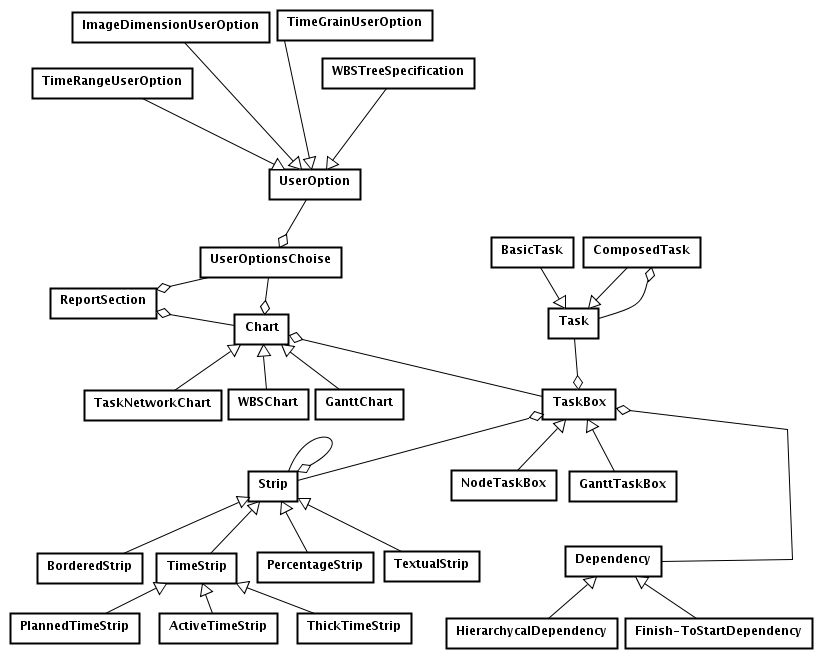
\includegraphics[width=1\textwidth]{../Milestone1-DomainModel/img/DomainModel.png}
	\caption{Overall UML diagram}
	\label{fig:overallDiagram} 
\end{figure}

Questo diagramma comprende tutti i concetti che abbiamo identificato durante la
prima iterazione del blocco di analisi. 

Nella figura abbiamo una visione di insieme che pu\`o essere utile a fini di
codifica e progettazione del piano delle prove. Finch\`e si rimane invece nella
sfera della progettazione (analisi inclusa) potrebbe produrre dei dubbi in
quanto propone molti concetti; mentre si sta cercando di raffinare le varie relazioni
secondo noi \`e necessaria una vista pi\`u in dettaglio di composizioni
di pochi concetti che sono legati tra loro, lasciando tutti gli altri ad una
loro commento separato.

Procediamo nel seguito del documento nella descrizione di piccole composizioni
in modo da chiarire i motivi per cui sono stati creati concetti e relazioni fra
essi.

\chapter{Aspects descriptions} 
% from here every document which is included with the input command must have a
% dedicated section whitin his body
\section{Task}
\label{sec:task}

\begin{figure}[h!] 
	\centering
	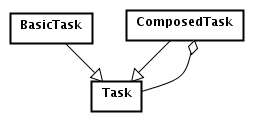
\includegraphics[width=0.4\textwidth]{../Milestone1-DomainModel/img/TaskDetail.png}
	\caption{task and its relations}
	\label{fig:task} 
\end{figure}

Molto probabilmente il concetto di \emph{Task} esiste gia nell'attuale
versione di \textbf{PMango 2.2.0}. Quello che abbiamo pensato \`e di introdurre
un \emph{glue layer} che ci permette di non apportare modifiche al codice
esistente di mango, ma lavorare con uno strato di intermezzo per essere il meno
intrusivi possibile e poter portare avanti il lavoro dipendendo solo dalle
nostri oggetti, facendo il minor riferimento al codice gia esistente.

Vogliamo rendere trasparente il concetto che un \emph{Task} sia un attivit\`a
singola (non scomponibile in sottoattivit\`a) che una attivit\`a scomposta. 

Costruiamo la relazione $\rightarrow$ che lega questi due concetti:
\begin{itemize}
  \item \emph{BasicTask} $\rightarrow$ attivit\`a di base, non ulteriormente
  scomponibili
  \item \emph{ComposedTask} $\rightarrow$ attivit\`a che sono composte da sotto
  attivit\`a
\end{itemize}
In questo modo possiamo trattare questi due tipi di attivit\`a in modo
interscambiabile e del tutto trasparente. Usando l'astrazione \emph{Task} non
ci importa se abbiamo una attivit\`a base o composta, in quanto cosi le abbiamo
portate ad avere interfaccie compatibili.

\section{TaskBox}
\label{sec:taskbox}

\begin{figure}[h!] 
	\centering
	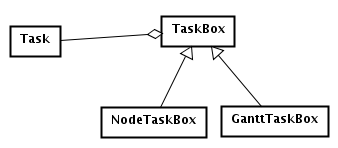
\includegraphics[width=0.5\textwidth]{../TaskBoxDetail.png}
	\caption{taskbox and its specializations}
	\label{fig:taskbox} 
\end{figure}

Il \emph{TaskBox} \`e la rappresentazione grafica di un
\emph{Task} (\autoref{fig:task}). Questo concetto astrae su queste
specializzazioni:
\begin{itemize}
\item \emph{GanttTaskBox} che ci permetter\`a di costruire la rappresentazione
in un \emph{GanttChart} conformi alle norme fissate nel documento di specifica.

\item \emph{NodeTaskBox} che ci permetter\`a di costruire la rappresentazione
in un \emph{WBSChart} e in \emph{TaskNetworkChart} alle norme fissate nel 
documento di specifica.
\end{itemize}

Abbiamo usato il principio di incapsulare il concetto che varia, modellando il
concetto astratto di \emph{TaskBox} per avere questi vantaggi:
\begin{itemize}
  \item non legare un \emph{Chart} specifico a una rappresentazione specifica
  \item aggiungere una nuova rappresentazione consiste nel modellarla e
  dichiarare che si tratta di una specializzazione di \emph{TaskBox}
  \item potremo cambiare a runtime il tipo di rappresentazione voluta nel
  disegno di un \emph{Chart}, magari inserire in un \emph{WBSChart} una
  rappresentazione pensata per i \emph{GanttChart}
\end{itemize}
\section{Strip}
\label{sec:strip}

\begin{figure}[h!] 
	\centering
	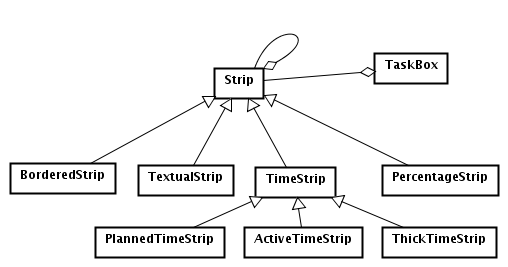
\includegraphics[width=0.7\textwidth]{../Milestone1-DomainModel/img/StripDetail.png}
	\caption{kinds of strips}
	\label{fig:strip} 
\end{figure}

La \emph{Strip} modella il concetto di ''striscia'': lo possiamo vedere come il
building block di pi\`u basso livello di tutta la nostra analisi. Si possono
osservare queste relazioni:
\begin{description}
  \item[TaskBox composition] \emph{TaskBox} contiene delle \emph{Strip},
  indipendentemente dalla rappresentazione dedicata ad uno specifico \emph{Chart}. Abbiamo costruito
  questa relazione in quanto per costruire un \emph{TaskBox} sar\`a sufficiente
  comporre un insieme di strip, tante quante sono necessarie per la corretta
  visualizzazione del \emph{Chart} che si sta disegnando.
  \item[russian doll] \emph{Strip} contiene a sua volta delle \emph{Strip}:
  questo \`e un concetto che pensiamo posso essere molto potente. Vogliamo rendere la
  \emph{Strip} un contenitore trasparente rispetto ad oggetti del suo stesso
  tipo. Questo ci permetter\`a di disegnare \emph{Strip} annidate, decidendo a
  runtime sia la \textbf{profondit\`a} di annidamento sia l'\textbf{ordine} con
  cui vengono annidate. Otteniamo cosi l'effetto di \emph{russian doll}, 
  dedicandoci a modellare solo alcune semplici specializzazioni di \emph{Strip},
  necessarie per l'implementazione delle notazioni richieste nel documento di specifica,
  limitandoci poi ad ottenere rappresentazioni complesse annidando quelle
  semplici.
  \item[specializations] abbiamo un primo livello di specializzazione:
  \begin{itemize}
    \item \emph{PercentageStrip} rappresenta un quantit\`a (l'intera
    \emph{Strip}) e la percentuale di comletamento (una parte di \emph{Strip}
    di colore diverso). Pu\`o essere composta da un \emph{GanttTaskBox} per
    indicare la percentuale di completamento relativa al \emph{Task}
    rappresentato.
    
    \item \emph{TextualStrip} permette di inserire delle stringhe di caratteri
    all'interno della \emph{Strip}. Questa possiamo utilizzarla ad esempio nel
    \emph{GanttChart} sulla destra della relativa \emph{TaskBox} per indicare
    l'effort oppure le risorse.
    
    \item \emph{BorderedStrip} permette di costruire un bordo, in modo che
    possiamo implementare la notazione per \emph{field} come richiesto per
    \emph{NodeTaskBox}
    
    \item \emph{TimeStrip} permettono di rappresentare informazioni relative a
    un intervallo di tempo. Queste sono i building blocks per
    \emph{GanttChart}. Possiamo specializzare ulteriormente questo concetto:
    \begin{itemize}
      \item \emph{PlannedTimeStrip} per costruire la parte superiore del
      \emph{GanttTaskBox} cdns
      \item \emph{ActualTimeStrip} per costruire la parte inferiore del
      \emph{GanttTaskBox} cdns      
      \item \emph{ThickTimeStrip} per costruire la parte superiore del
      \emph{GanttTaskBox} nel caso la rappresentazione sia di un
      \emph{ComposedTask} cdns
    \end{itemize}
  \end{itemize}
\end{description}

\section{Chart}
\label{sec:chart}

\begin{figure}[h!] 
	\centering
	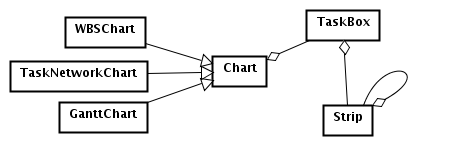
\includegraphics[width=0.6\textwidth]{../ChartDetail.png}
	\caption{chart and building blocks}
	\label{fig:chart} 
\end{figure}

Il \emph{Chart} modella il concetto di grafico generico. Per implementare la
specifica abbiamo queste specializzazioni:
\begin{itemize}
  \item \emph{GanttChart} che permette di avere la rappresentazione delle
  attivit\`a nel tempo
  \item \emph{WBSChart} per avere una vista gerarchica delle attivit\`a e di
  come sono state raffinate e decomposte in sotto attivit\`a
  \item \emph{TaskNetworkChart} per rappresentare le dipendenze di tipo
  \emph{finish-to start} fra coppie di attivit\`a
\end{itemize}

Per costruire un \emph{Chart} \`e sufficiente assemblare \emph{TaskBox} in base
ad alcune preferenze del client che richiede la generazione.

\section{Dependency}
\label{sec:dependency}

\begin{figure}[h!] 
	\centering
	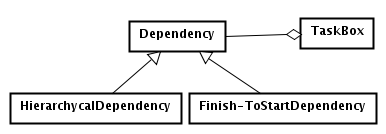
\includegraphics[width=0.5\textwidth]{../Milestone1-DomainModel/img/DependencyDetail.png}
	\caption{dependencies}
	\label{fig:dependencies} 
\end{figure}

\emph{Dependency} modella il tipo di dipendenze che possiamo rappresentare in
un \emph{Chart}. Per implementare la specifica abbiamo bisogno di incapsulare
queste varianti:\footnote{dire in quali Chart vengono utilizzate}
\begin{itemize}
  \item \emph{Finish-ToStartDependency}: siano $a, b$ due \emph{Task} tali
  che $b$ non pu\`o iniziare finch\'e $a$ non sia completato. Questa relazione
  \`e catturata da questa specializzazione.
  \item \emph{HierarchycalDependency}: siano $a, b_{i}$ con $i= 1,\ldots,n \in
  N$, \emph{Task}s tali che $a$ \`e scoposto in $b_{i}$ \emph{Task}. Questa
  relazione \`e catturata da questa specializzazione.
\end{itemize}
\section{UserOption}
\label{sec:userOption}

\begin{figure}[h!] 
	\centering
	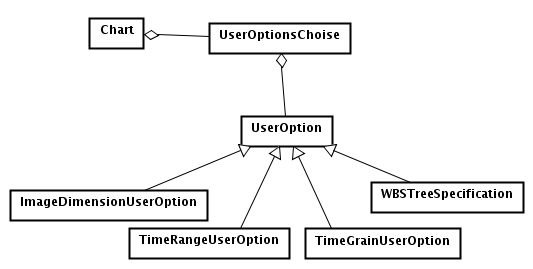
\includegraphics[width=0.7\textwidth]{../Milestone1-DomainModel/img/UserOptionDetail.png}
	\caption{UserOptions and choice}
	\label{fig:userOption} 
\end{figure}

Quando un generico client (potrebbe essere sia una persona fisica che un
oggetto astratto) della nostra implementazione della specifica vuole generare
un \emph{Chart} pu\`o guidare la generazione decidendo alcuni fattori che sono
di suo interesse. Questi fattori vengono modellati dal concetto di
\emph{UserOption}.

Ogni \emph{Chart} espone una lista di \emph{UserOption} per dare al client la
possibilit\`a di esprimere quali informazioni guidare. Questa lista varia da
\emph{Chart} a \emph{Chart}\footnote{creare un reference dove vengono mappate
questa relazione: potrebbe essere un appendici di questo documento??}.

Il concetto di lista di \emph{UserOption} \`e catturato in
\emph{UserOptionsChoice}.

Procediamo per passi: nelle prossime subsection osserviamo due aspetti che
trattarli insieme potrebbe non essere sufficiente per esporli in modo chiaro.

\subsection{\emph{UserOption}'s Instances}
\label{subsec:UserOptionInstances}
Questa \`e stata una decisione non molto facile da prendere. Il problema \`e
questo: nella specifica abbiamo che per ogni \emph{Chart} il committente ha
dichiarato quali \emph{UserOption} mostrare. Queste per\`o non rappresentano un
concetto che vogliamo catturare nel nostro modello, ma allo stesso tempo sono
\emph{istanze} (un insieme discreto quindi) di elementi che fissa il
committente.

Per questo motivo decidiamo di codificare questo insieme discreto in questo
documento e la successiva enumerazione \`e da considerarsi parte integrante del
diagramma inserito come figura.

Rappresentiamo il concetto espresso sopra indicando due descrizioni con questa
struttura di codifica:
\begin{itemize}
  \item \emph{istanze}, dove inseriamo tutte le possibili \emph{UserOption} che
  non possono essere ancora raffinate
  \item \emph{specializzazioni} dove inseriamo tutte le possibili
  specializzazioni di \emph{UserOption} che possono essere ancora raffinate,
  ripetendo in modo ricorsivo questa struttura di codifica
\end{itemize}

Le successive descrizioni sono relative al concetto di \emph{UserOption}:
\begin{description}
  \item[istanze]\footnote{inserire qui la il mapping sui vari Chart?}
  \emph{WBSExplosionLevelUserOption, ActualTimeFrameOption, CompletitionBarOption, \\ PlannedDataOption, ActualDataOption,
  AlertMarkUserOption, ReplicateArrowUserOption, FindCriticalPathUserOption,
  WBSUserSpecificationUserLevel, \\WBSUserSpecificationUserLevel,
  ResourcesDetailsOption, TaskNameOption, CompleteDiagramUserOptions,
  ShowDependencies}
  \item[specializzazioni] \quad
  \begin{itemize}
    \item \emph{WBSTreeSpecification}
    \begin{description}
  \item[istanze] \emph{LevelSpecification, UserCustomSpecification}
  \item[specializzazioni] nessuna
\end{description}

\item \emph{TimeGrainUserOption}
    \begin{description}
  \item[istanze] \emph{HourlyGrain, DailyGrain, WeaklyGrain, MonthlyGrain,
  AnnuallyGrain}
  \item[specializzazioni] nessuna
\end{description}

\item \emph{ImageDimensionUserOption}
    \begin{description}
  \item[istanze] \emph{CustomDim, FitInWindowDim, OptionalDim, DefaultDim}
  \item[specializzazioni] nessuna
\end{description}

\item \emph{TimeRangeUserOption}
    \begin{description}
  \item[istanze] \emph{CustomRange, WholeProjectRange, FromStartRange, ToEndRange}
  \item[specializzazioni] nessuna
\end{description}

  \end{itemize}
\end{description}

\subsection{\emph{UserOptionsChoice}}
Questo concetto \`e, secondo la nostra analisi, molto importante in quanto ci
permette di astrarre dal client che richiede una generazione.

Il motivo per cui abbiamo introdotto questo concetto \`e di poter lavorare lato
server usando \emph{UserOptionsChoice} per controllare quali informazioni il
client vuole guidare. In questo modo non siamo vincolati ad accedere ai dati
inviati per \emph{POST, GET} dalla form HTML, ma possiamo direttamente guardare
in \emph{UserOptionsChoice}. Queste ci permette di disaccopiare il processo di
generazione della maschera di input di una pagina HTML. 

Se vogliamo utilizzare il processo di generazione (che comunque \`e
server side) scrivendo un programma client (GUI o da riga di comando) che
costruisce una HTML request ad hoc (dovremo definire una grammatica e
attribuire la semantica ai contesti, questo \`e necessario, non ch\`e scrivere 
un parser), usando \emph{UserOptionsChoice} e il suo disaccoppiamento ci sar\`a
possibile farlo. 

Una volta ricevuta la response possiamo maneggiare la pagina
inviata come una response HTML valida e usarla per i nostri obiettivi (possiamo
rihiedere l'immagina generata, o il file PDF generato, salvandolo in
locale, oppure visualizzando lo stesso con un browser, ma possiamo anche
inserire in un db oppure farci dei test sopra\ldots).

Dovremo quindi costruire un oggetto che si incarica di costruire
\emph{UserOptionsChoice} in base al tipo di richiesta ricevuta (da una pagina
html come \`e il caso di PMango, oppure una richiesta da un client indipendente
scritto in un qualche linguaggio). Una volta costruito l'insieme delle
\emph{UserOption} \`e possibile iniziare la generazione. Questo sar\`a delegato
alla fase di progettazione.

\section{ReportSection}
\label{sec:reportSection}

\begin{figure}[h!] 
	\centering
	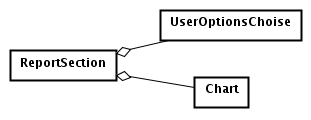
\includegraphics[width=0.5\textwidth]{../ReportSectionDetail.png}
	\caption{report section}
	\label{fig:reportSection} 
\end{figure}

Abbiamo da implemetare un requisito che vuole la possibilit\`a di aggiungere
alla reportistica un determinato \emph{Chart} con le relative \emph{UserOption}
scelte dall'utente. Modelliamo quindi il concetto di \emph{ReportSection} per
realizzare questo requisito. Come si vede dalla figura, \emph{ReportSection}
associa \emph{Chart} e \emph{UserOptionChoice}. Utilizziamo direttamente la
lista delle scelte\footnote{che viene costruita lato server} in modo da non
doverla costruire nella funzionalit\`a di assemblamento del report.



\end{document}